\section{Математическое описание}

\subsection{Связный ациклический граф}
Графом $G(V,E)$ называется совокупность двух множеств — непустого множества $V$ (множества вершин) и множества $E$ двухэлементных подмножеств множества $V$ ($E$ — множество рёбер):
\[
G(V, E) = \langle V; E \rangle, \quad V \neq \varnothing, \quad E \subset 2^V \land \forall e \in E \ (|e| = 2).
\]
Маршрутом в графе называется чередующаяся последовательность вершин и рёбер, начинающаяся и кончающаяся вершиной, в которой любые два соседних элемента инцидентны, причём однородные элементы (вершины, рёбра) через один смежны или совпадают. Если все рёбра различны, то маршрут называется цепью. Если все вершины (а значит, и рёбра) различны, то маршрут называется простой цепью. Замкнутая цепь называется циклом, замкнутая простая цепь называется простым циклом. Число циклов в графе $G$ обозначается $z(G)$. Граф без циклов называется ациклическим.

Говорят, что две вершины в графе связаны, если существует соединяющая их (простая) цепь. Граф, в котором все вершины связаны, называется связным.

\subsection{Распределение Чампернауна}
Распределение Чампернауна — это непрерывное распределение вероятностей, применяемое для моделирования данных. 

Для генерации случайных чисел, имеющих распределение Чампернауна, используется метод обратного преобразования. Если $r$ — равномерно распределённое на интервале $(0,1)$ случайное число, то величина
\[
x = \mu + \frac{1}{\alpha} \ln \operatorname{tg}\left(\frac{\pi r}{2}\right)
\]
подчиняется распределению Чампернауна с параметрами $\mu$ и $\alpha$. В данной работе используется именно эта формула для генерации случайных чисел.

На рис.~\ref{fig:champ} представлена гистограмма на 1000 значений для распределения Чампернауна для констант $mu = 1$ и $alpha = 1.57$ используемых в программе.

\begin{figure}[H]
	\centering
	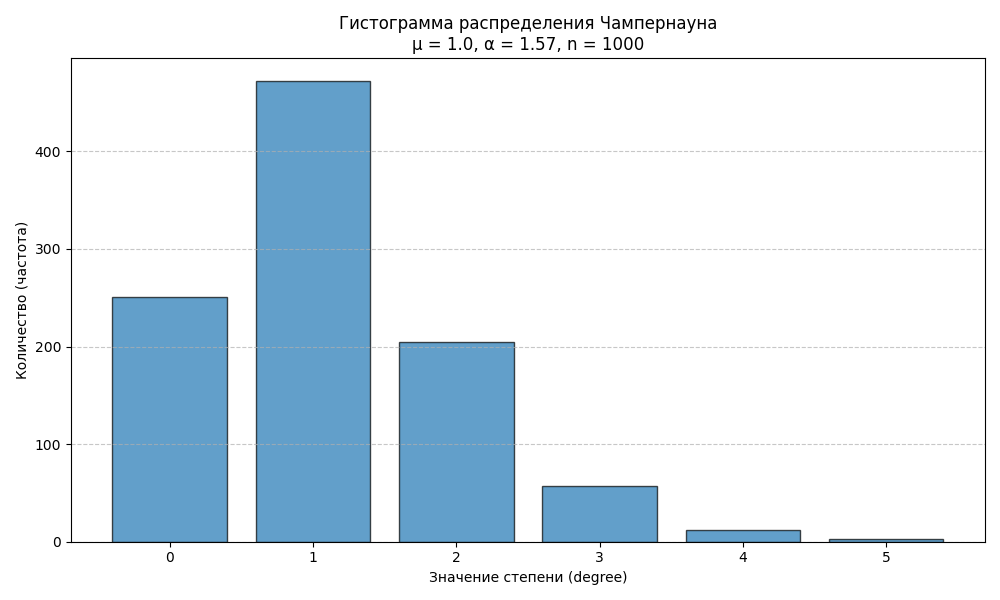
\includegraphics[width=0.9\textwidth]{pic/Raspr.png}
	\caption{Гистограмма распределения Чампернауна для констант $\mu = 1$, и $\alpha = 1.57$}
	\label{fig:champ}
\end{figure}

\subsection{Метод Шимбелла}
Метод Шимбелла позволяет находить кратчайшие или максимальные пути между вершинами, состоящие из заданного количества рёбер. Операции в методе:
\begin{enumerate}
	\item Умножение двух величин $a$ и $b$ при возведении матрицы в степень соответствует их алгебраической сумме: \\ $a \cdot b = b \cdot a \Rightarrow a + b = b + a$, \\ $a \cdot 0 = 0 \cdot a \Rightarrow a + 0 = 0$.
	\item Операция сложения двух величин $a$ и $b$ заменяется выбором минимального (максимального) элемента, то есть: \\ $a + b = b + a = \min(\max)\{a, b\}$.
\end{enumerate}
С помощью операций Шимбелла длины кратчайших или максимальных путей между всеми вершинами определяются возведением в степень весовой матрицы, содержащей веса рёбер. Степень равна количеству рёбер в искомом пути. Сложность метода Шимбелла составляет $O(kn^3)$, где $n$ — количество вершин, а $k$ — длина пути (количество рёбер).

\subsection{Поиск количества маршрутов от одной вершины до другой}
Пусть дан простой граф $G = (V, A)$, матрица смежности которого есть $A = (a_{ij})_{n\times n}$, где $a_{ij}=1 \Leftrightarrow (i,j) \in A$. Матрица $R(G) = E \lor A \lor A^2 \lor \dots \lor A^{n-1}$ есть матрица достижимости, где $E$ – единичная матрица. Количество маршрутов длины $k$ между вершинами определяется элементами $A^k$. Сложность поиска количества маршрутов длины $k$ между вершинами через возведение матрицы смежности в степень составляет $O(kn^3)$, где $n$ — число вершин.


\subsection{Точки сочленения графа}
Вершина графа называется точкой сочленения, или разделяющей вершиной, если её удаление увеличивает число компонент связности. Пусть \( G(V, E) \) — связный граф и \( v \in V \). Тогда следующие утверждения эквивалентны:
\begin{enumerate}
	\item \( v \) — точка сочленения.
	\item \( \exists u, w \in V \ (u \neq w \ \& \ \forall \langle u, w \rangle_G \ (v \in \langle u, w \rangle)) \).
	\item \( \exists U, W \ (U \cap W = \varnothing \ \& \ U \cup W = V - v \ \& \ \forall u \in U, w \in W \ (\forall \langle u, w \rangle_G \ (v \in \langle u, w \rangle_G)) \).
\end{enumerate}

 Для их поиска используется модифицированный обход в глубину (DFS), в ходе которого для каждой вершины вычисляются глубина входа в дереве обхода и наименьшая глубина, достижимая из её поддерева по обратным рёбрам. Корневая вершина является точкой сочленения, если у неё не менее двух детей в дереве DFS. Не корневая вершина $v$ является точкой сочленения, если существует хотя бы один её потомок $u$, из поддерева которого нет обратного ребра в предка $v$ или более раннюю вершину. Сложность алгоритма поиска точек сочленения на основе обхода в глубину составляет $O(n + m)$, где $n$ — количество вершин, а $m$ — количество рёбер.
 
\subsection{Алгоритм Дейкстры}
Алгоритм Дейкстры находит оптимальные маршруты и их длину между одной конкретной вершиной (источником $s$) и вершиной $t$ (всеми остальными вершинами) (ор)графа. Недостаток алгоритма: некорректно работает, если граф имеет рёбра (дуги) отрицательного веса. Сложность алгоритма Дейкстры составляет $O(p^2)$.

Принцип работы алгоритма: каждой вершине присваивается метка — текущее известное расстояние от источника. В начале источник получает постоянную метку $0$, а все остальные — временные метки $\infty$. На каждом шаге из всех временных меток выбирается вершина с наименьшим значением, её метка становится постоянной. Затем для всех непосредственных последователей этой вершины временные метки обновляются по правилу $d_{\text{нов}}(x_i) = \min\{d_{\text{стар}}(x_i), d(\tilde{x}) + \omega(\tilde{x}, x_i)\}$, где $\tilde{x}$ - текущая вершина (та, чья метка только что стала постоянной), а $\omega(\tilde{x}, x_i)$ - вес дуги от $\tilde{x}$ к $x_i$. Процесс повторяется, пока постоянная метка не будет присвоена каждой вершине графа; на выходе получаем вектор длин кратчайших путей от $s$. После этого кратчайший путь восстанавливается обратным ходом: начиная с $t$, на каждом шаге находится вершина $x_i$, удовлетворяющая $d(\tilde{x}) = d(x_i) + \omega(x_i, \tilde{x})$, и включается дуга $(x_i, \tilde{x})$ в путь; процесс продолжается до достижения источника $s$. Псевдокод алгоритма представлен на рисунке.

\begin{figure}[H]
	\centering
	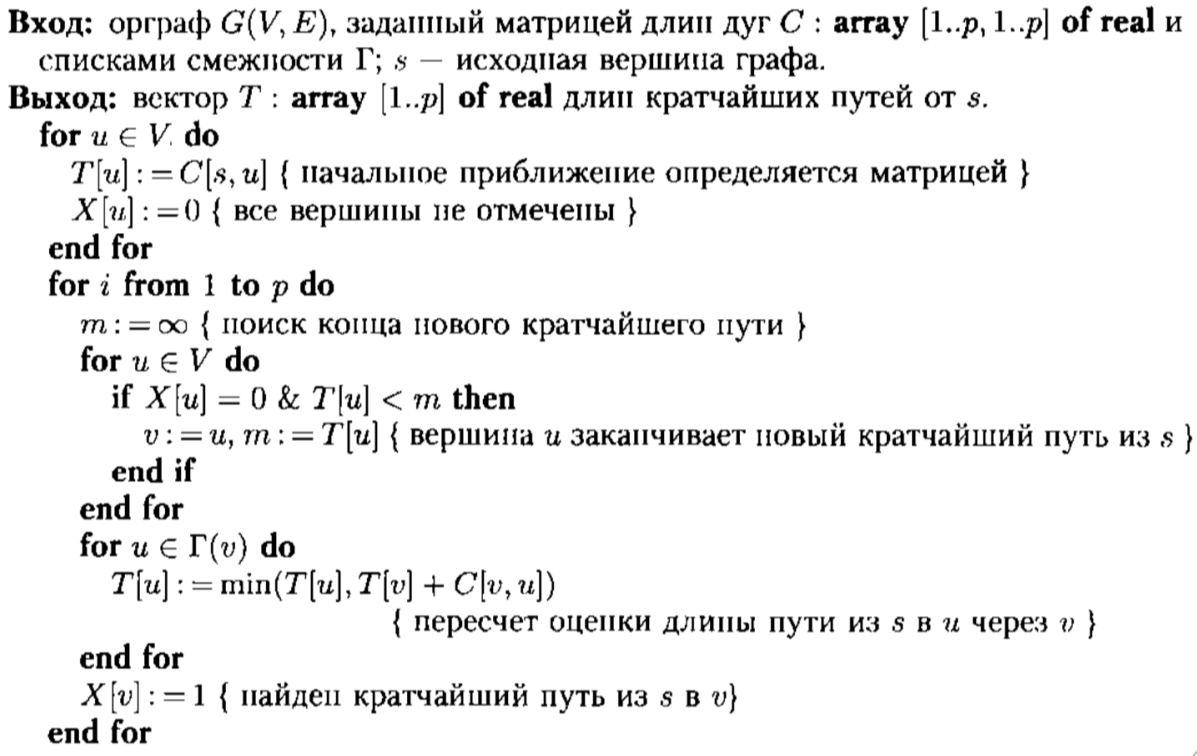
\includegraphics[width=0.9\textwidth]{pic/Deikstra.png}
	\caption{Псевдокод построения дерева кратчайших путей.}
	\label{fig:Deikstra}
\end{figure}


\subsection{Алгоритм Форда-Фалкерсона}
Потоком в сети \( S = (G; c) \), где \( G = (V, E) \), называется такая функция \( f : E \to \mathbb{R}_+ \), приписывающая каждой дуге \( e \in E \) неотрицательное число \( f(e) \), называемое \textbf{потоком} по этой дуге \( e \), для которой выполняются свойства:

\begin{enumerate}
	\item для каждой дуги \( e \in E \) верно \( f(e) \leq c(e) \), т.е. поток по любой дуге не превышает пропускную способность этой дуги;
	\item для каждой вершины \( v \in V \), \( v \neq s, t \), верно
	\[
	D_f(v) = \sum_{e \in A(v)} f(e) - \sum_{e \in B(v)} f(e) = 0,
	\]
	где $A(v)$ — дуги входящие в $v$, а $B(v)$ — дуги исходящие из $v$, т.е. поток, входящий в любую вершину, кроме источника и стока, без остатка выходит из нее (сохранение потока).
\end{enumerate}

При этом неотрицательное число \( p_f = \sum_{e \in B(s)} f(e) \) называется величиной потока \( f \).

Алгоритм Форда-Фалкерсона находит максимальный поток в направленной сети с источником $s$ и стоком $t$. Ключевую роль играют пропускные способности рёбер и остаточная сеть. Алгоритм работает, последовательно увеличивая поток вдоль увеличивающих путей в остаточном графе, пока такие пути существуют.

\textbf{Алгоритм:}
\begin{enumerate}
	\item Для каждого ребра $(u \to v)$ устанавливаем поток $f(u, v) = 0$. Строим остаточную сеть $G_f$, где каждому ребру $(u \to v)$ с пропускной способностью $c(u, v)$ соответствуют прямое ребро с остаточной пропускной способностью $c_f(u, v) = c(u, v) - f(u, v)$ и обратное ребро с остаточной пропускной способностью $c_f(v, u) = f(u, v)$.
	\item Находим любой путь от $s$ до $t$ в остаточной сети $G_f$, где все рёбра имеют положительную остаточную пропускную способность. Если такого пути нет — алгоритм завершён, текущий поток максимален.
	\item Находим минимальную остаточную пропускную способность $c_f$ на выбранном пути (это и есть возможное увеличение потока). Для каждого ребра $(u \to v)$ на пути: увеличиваем поток $f(u, v) \mathrel{+}= c_f$, уменьшаем остаточную пропускную способность $c_f(u, v) \mathrel{-}= c_f$, увеличиваем остаточную пропускную способность обратного ребра $c_f(v, u) \mathrel{+}= c_f$.
	\item Возвращаемся к шагу 2 и ищем новый увеличивающий путь в обновлённой остаточной сети.
\end{enumerate}

В данной работе для поиска максимального потока используется реализация \\ Эдмондса–Карпа, которая является частным случаем метода Форда–Фалкерсона. Отличие от описанного выше алгоритма заключается в способе выбора увеличивающего пути: на каждой итерации путь ищется с помощью поиска в ширину (BFS). Это гарантирует, что каждый найденный путь будет кратчайшим по числу рёбер в остаточной сети. Благодаря этому трудоёмкость алгоритма становится полиномиальной и составляет $O(nm^2)$, где $n$ — число вершин, $m$ — число рёбер (вместо $O(nmU)$ для исходного метода Форда–Фалкерсона, где $U$ — максимальная пропускная способность сети).

\subsection{Алгоритм поиска заданного потока минимальной стоимости}

Рассматривается задача определения потока заданной величины $\vartheta$ от источника $s$ к стоку $t$ в сети $G = (S, U, \Omega, D)$, где каждая дуга $(x_i, x_j) \in U$ характеризуется пропускной способностью $c(x_i, x_j) \in \Omega$ и неотрицательной стоимостью $d(x_i, x_j) \in D$ пересылки единицы потока из $x_i$ в $x_j$. Цель — минимизировать суммарную стоимость
\[
\sum_{(x_i, x_j) \in U} d(x_i, x_j) \cdot \varphi(x_i, x_j)
\]
при ограничениях:
\begin{enumerate}
	\item $0 \leq \varphi(x_i, x_j) \leq c(x_i, x_j)$ для всех $(x_i, x_j) \in U$;
	\item для источника $s$: $\displaystyle \sum_{x_i \in S} \varphi(s, x_i) - \sum_{x_j \in S} \varphi(x_j, s) = \vartheta$;
	\item для стока $t$: $\displaystyle \sum_{x_i \in S} \varphi(t, x_i) - \sum_{x_j \in S} \varphi(x_j, t) = -\vartheta$;
	\item для любой другой вершины $x_k \neq s, t$: $\displaystyle \sum_{x_i \in S} \varphi(x_k, x_i) - \sum_{x_j \in S} \varphi(x_j, x_k) = 0$ (сохранение потока).
\end{enumerate}

Если $\vartheta > \varphi_{\max}$, где $\varphi_{\max}$ — величина максимального потока в сети, то решения не существует. В противном случае требуется найти поток минимальной стоимости.

В данной работе для нахождения потока минимальной стоимости заданной величины используется алгоритм последовательных кратчайших путей с потенциалами. Идея метода заключается в итеративном увеличении потока вдоль кратчайших по стоимости путей в остаточной сети. Для учёта возможных отрицательных стоимостей обратных дуг применяются приведённые стоимости с использованием потенциалов вершин, что позволяет использовать алгоритм Дейкстры для поиска кратчайшего пути на каждой итерации.

Построение остаточной сети (модифицированной относительно текущего потока $\varphi$):
Пусть $G = (S, U, \Omega, D)$ — исходная сеть, а $\varphi$ — некоторый поток. Модифицированная сеть $\tilde{G} = (\tilde{S}, \tilde{U}, \tilde{\Omega}, \tilde{D})$ строится следующим образом:
\begin{enumerate}
	\item $\tilde{S} = S$ (множество вершин не изменяется);
	\item $\tilde{U} = U \cup V$, где $V$ — множество фиктивных дуг (обратных);
	\item для каждой дуги $(x_i, x_j) \in U$, по которой проходит положительный поток ($\varphi(x_i, x_j) > 0$), добавляется обратная дуга $(x_j, x_i)$ с параметрами:
	\[
	\tilde{c}(x_j, x_i) = \varphi(x_i, x_j), \qquad \tilde{d}(x_j, x_i) = -d(x_i, x_j);
	\]
	\item для всех ненасыщенных дуг (включая те, по которым поток нулевой) полагается:
	\[
	\tilde{c}(x_i, x_j) = c(x_i, x_j) - \varphi(x_i, x_j), \qquad \tilde{d}(x_i, x_j) = d(x_i, x_j);
	\]
	\item для насыщенных дуг ($\varphi(x_i, x_j) = c(x_i, x_j)$) полагается:
	\[
	\tilde{c}(x_i, x_j) = 0, \qquad \tilde{d}(x_i, x_j) = \infty.
	\]
\end{enumerate}

\paragraph{Алгоритм:}
\begin{enumerate}
	\item Начальный поток полагается нулевым, потенциалы всех вершин равны нулю.
	\item На каждой итерации в остаточной сети с помощью алгоритма Дейкстры ищется кратчайший путь из $s$ в $t$ по приведённым стоимостям
	\[
	\tilde{d}_{\text{прив}}(u, v) = \tilde{d}(u, v) + \text{pot}(u) - \text{pot}(v),
	\]
	которые неотрицательны при корректном обновлении потенциалов.
	\item Если путь не найден, алгоритм завершается — достигнут максимальный поток.
	\item Вдоль найденного пути определяется максимально возможное увеличение потока $\delta$ (минимальное из остаточных пропускных способностей дуг на пути и оставшегося требуемого потока $\vartheta - \text{достигнутый поток}$).
	\item Поток увеличивается на $\delta$ вдоль всех дуг пути (прямые дуги увеличиваются, обратные — уменьшаются). Соответственно обновляются остаточные пропускные способности в модифицированной сети.
	\item Суммарная стоимость увеличивается на $\delta \cdot \sum \tilde{d}(u,v)$ по дугам пути (с учётом знака для обратных дуг).
	\item Потенциалы вершин обновляются: $\text{pot}(v) \leftarrow \text{pot}(v) + \text{dist}(v)$ для всех достижимых вершин $v$.
	\item Шаги 2–7 повторяются, пока не будет достигнут требуемый поток $\vartheta$ или не останется увеличивающих путей.
\end{enumerate}

Сложность алгоритма составляет $O(\vartheta n^2)$ при использовании Дейкстры с матрицей смежности, где $n$ — число вершин, $\vartheta$ — величина целевого потока.

\subsection{Матричная теорема Кирхгофа}

Пусть \( G(V, E) \) — граф. Остовный подграф графа \( G(V, E) \) — это подграф, содержащий все вершины. Остовный подграф, являющийся деревом, называется остовом.

Остов определяется множеством рёбер, поскольку вершины остова — это вершины исходного графа. Несвязный граф не имеет остова. Связный граф может иметь много остовов.

Определим матрицу Кирхгофа \( B = B(G) = (\beta_{ij})_{n \times n} \) неориентированного графа \( G \) порядка \( n \). Положим
\[
B(G) = 
\begin{pmatrix}
	\deg v_1 & 0 & \cdots & 0 \\
	0 & \deg v_2 & \cdots & 0 \\
	\vdots & \vdots & \ddots & \vdots \\
	0 & 0 & \cdots & \deg v_n
\end{pmatrix} - A(G),
\]
где \( A(G) \) — матрица смежности графа \( G \). Иными словами,
\[
\beta_{ij} =
\begin{cases} 
	-1, & \text{если } i \neq j \text{ и } v_i \text{ смежна с } v_j, \\
	0, & \text{если } i \neq j \text{ и } v_i \text{ не смежна с } v_j, \\
	\deg v_i, & \text{если } i = j.
\end{cases}
\]

\textbf{Теорема Кирхгофа.}  
Число остовных деревьев в связном графе \( G \) порядка \( n \geq 2 \) равно алгебраическому дополнению любого элемента матрицы Кирхгофа \( B(G) \). Кроме того, все алгебраические дополнения матрицы Кирхгофа равны между собой.

Сложность вычисления числа остовных деревьев по матричной теореме Кирхгофа составляет $O(n^3)$, где $n$ — число вершин графа.

\subsection{Алгоритм Борувки}
Алгоритм Борувки используется для нахождения кратчайшего остова (минимального остовного дерева) связного взвешенного графа. Сложность алгоритма Борувки составляет $O(m\log{n})$, где $n$ — количество вершин в графе, а $m$ — количество рёбер. Пусть \(T\) — подграф графа \(G\). Изначально \(T\) содержит все вершины \(G\) и не содержит рёбер. Далее выполняется следующий процесс:

\begin{enumerate}
	\item Пока \(T\) не является деревом (что эквивалентно условию: число компонент связности $k = 1$), для каждой компоненты связности текущего леса \(T\) находится ребро минимального веса, которое соединяет вершину данной компоненты с вершиной, не принадлежащей этой компоненте.
	\item В \(T\) добавляются все рёбра, которые оказались минимальными хотя бы для одной компоненты связности.
\end{enumerate}

Полученный в результате граф \(T\) является минимальным остовным деревом исходного графа. Следует учитывать, что алгоритм может работать некорректно при наличии рёбер одинакового веса. Например, в полном графе из трёх вершин, где все рёбра имеют вес \(1\), в \(T\) могут быть добавлены все три ребра, что приведёт к циклу. Чтобы избежать этой проблемы, при выборе минимального ребра среди равных по весу следует выбирать ребро с наименьшим номером.

\subsection{Код Прюфера}
Код Прюфера устанавливает взаимно однозначное соответствие между деревьями с $p$ вершинами и последовательностями длины $p-2$ из чисел $1,\dots,p$ (с возможными повторениями). Это позволяет экономно хранить структуру дерева.

\textbf{Построение кода (кодирование):}
Исходное дерево имеет вершины, занумерованные числами от $1$ до $p$ (произвольным образом). На каждом шаге из текущего дерева выбирается висячая вершина (степени $1$) с наименьшим номером, в код записывается номер единственного соседа этой вершины, после чего выбранная вершина удаляется. Процесс повторяется $p-2$ раза; последнее оставшееся ребро восстанавливается однозначно, поэтому его можно не хранить.

\textbf{Восстановление дерева по коду (декодирование):}
Дан код $A[1..p-2]$ (последовательность чисел от $1$ до $p$). Множество ещё не использованных вершин $B$ изначально содержит все номера $1,\dots,p$. Для $i$ от $1$ до $p-2$ выбирается наименьшая вершина $v$ из $B$, которая не встречается в оставшейся части кода $A[i], A[i+1], \dots, A[p-2]$, и добавляется ребро $(v, A[i])$, после чего $v$ удаляется из $B$. По завершении цикла в $B$ остаются две вершины, которые соединяются последним ребром.

В лабораторной работе при кодировании и декодировании необходимо сохранять не только номера вершин, но и веса рёбер, чтобы после декодирования остов имел те же веса. Сложность построения кода Прюфера (кодирование) составляет $O(n)$, где $n$ — число вершин. Декодирование также выполняется за $O(n)$.

\subsection{Алгоритм нахождения минимальной раскраски графа}
Раскраской графа называется приписывание цветов (натуральных чисел) его вершинам такое, что никакие две смежные вершины не получают одинаковый цвет. Множество вершин одного цвета образует независимое множество (одноцветный класс). Наименьшее возможное число цветов есть хроматическое число \(\chi(G)\), при этом выполняется \(\chi(G) \le 1 + \Delta(G)\), где \(\Delta(G)\) — максимальная степень вершины.

В данной работе для построения допустимой раскраски используется улучшенный алгоритм последовательного раскрашивания. Его идея — сначала упорядочить вершины по невозрастанию их степеней. Затем алгоритм работает по цветам: на первом шаге все ещё не раскрашенные вершины просматриваются в указанном порядке, и если ни один сосед вершины ещё не покрашен в текущий цвет, вершина получает этот цвет и удаляется из дальнейшего рассмотрения. Когда все возможные вершины покрашены в текущий цвет, алгоритм переходит к следующему цвету и повторяет процесс. Так продолжается, пока все вершины не получат цвета. Полученная раскраска является допустимой, однако не обязательно минимальной; тем не менее эвристика с сортировкой по степени часто даёт результат, близкий к оптимальному. Сложность улучшенного последовательного алгоритма раскраски графа $O(n^2)$, где $n$ — число вершин.

\subsection{Эйлеров граф}
Если граф имеет цикл (не обязательно простой), содержащий все рёбра графа, то такой цикл называется эйлеровым циклом, а граф называется эйлеровым. Если граф имеет цепь, содержащую все рёбра, то такая цепь называется эйлеровой цепью, а граф — полуэйлеровым. Эйлеров цикл содержит каждое ребро ровно один раз, а вершины могут повторяться. Эйлеровым может быть только связный граф.

Справедлива теорема Эйлера: для связного нетривиального графа следующие утверждения эквивалентны:
\begin{enumerate}
	\item Граф является эйлеровым.
	\item Каждая вершина графа имеет чётную степень.
	\item Множество рёбер графа можно разбить на простые циклы.
\end{enumerate}

Для построения эйлерова цикла в эйлеровом графе используется алгоритм Флери. Он работает следующим образом.

\begin{enumerate}
	\item Создаётся пустой стек для хранения вершин.
	\item Выбирается произвольная вершина и помещается в стек.
	\item Пока стек не пуст, выполняется:
	\begin{itemize}
		\item $v$ — вершина на вершине стека.
		\item Если у вершины $v$ нет смежных рёбер, то $v$ извлекается из стека и добавляется в эйлеров цикл.
		\item Иначе выбирается любая смежная вершина $u$, ребро $(v, u)$ удаляется из графа, а вершина $u$ помещается в стек.
	\end{itemize}
\end{enumerate}

Ключевая особенность алгоритма заключается в том, что при наличии выбора следует избегать рёбер, являющихся мостами, поскольку их удаление может привести к невозможности пройти оставшиеся рёбра. Ребро является мостом, если его удаление увеличивает количество компонент связности графа; проверка выполняется с помощью поиска в ширину (BFS) до и после временного удаления ребра. Если других рёбер нет, мост может быть пройден.

Ниже представлен псевдокод алгоритма:

\begin{figure}[H]
	\centering
	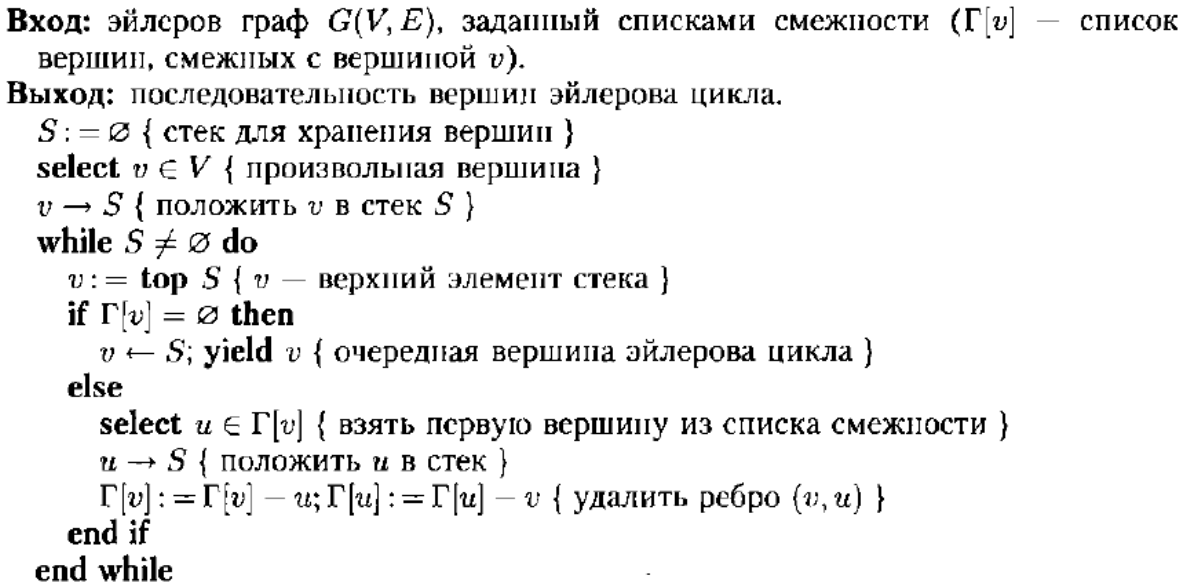
\includegraphics[width=0.9\textwidth]{pic/Fleri.png}
	\caption{Псевдокод алгоритма Флери.}
	\label{fig:Fleri}
\end{figure}

Сложность проверки существования эйлерова цикла (проверка чётности степеней) составляет $O(n)$, где $n$ — число вершин. Сложность построения эйлерова цикла алгоритмом Флери составляет $O(m^2)$, где $m$ — количество рёбер.

\subsection{Разрез графа}
Разрезом связного графа называется множество рёбер, удаление которых делает граф несвязным. Любое разбиение множества вершин $V$ на два непустых подмножества: $V_1 \neq \varnothing и V_2 \neq \varnothing, V_1 \cap V_2 = \varnothing, V_1 \cup V_2 = V$ определяет разрез $S = \{ (v_1, v_2) \in E ~|~ v_1 \in V_1 ~\&~ v_2 \in V_2 \}$

\subsection{Фундаментальная система разрезов}
Пусть $T(V,E_T)$ — некоторый остов связного графа $G(V,E)$. Для каждого ребра остова $e \in E_T$ рассмотрим разрез $S_e$, определяемый следующим образом. Поскольку $e$ является мостом в дереве $T$, его удаление разбивает множество вершин $V$ на два непустых подмножества $V_1$ и $V_2$ ($V_1 \cup V_2 = V$, $V_1 \cap V_2 = \varnothing$). Включим в разрез $S_e$ само ребро $e$ и все хорды остова $T$ (то есть рёбра графа $G$, не принадлежащие $T$), соединяющие вершины из $V_1$ с вершинами из $V_2$. Иными словами, $S_e = E(V_1, V_2)$ — множество всех рёбер графа $G$ между $V_1$ и $V_2$, которое является простым разрезом. Совокупность разрезов $\{S_e\}_{e \in E_T}$ называется фундаментальной системой разрезов графа $G$ относительно остова $T$. Количество разрезов в этой системе совпадает с числом рёбер остова и равно коциклическому рангу графа, обозначаемому $m^*(G)$. Сложность построения фундаментальной системы разрезов составляет $O(n(n + m))$, где $n$ — число вершин, $m$ — число рёбер. Для одного разреза — $O(n + m)$.